% Options for packages loaded elsewhere
\PassOptionsToPackage{unicode}{hyperref}
\PassOptionsToPackage{hyphens}{url}
\PassOptionsToPackage{dvipsnames,svgnames,x11names}{xcolor}
%
\documentclass[
  12pt,
  letterpaper,
  DIV=11,
  numbers=noendperiod]{scrartcl}

\usepackage{amsmath,amssymb}
\usepackage{setspace}
\usepackage{iftex}
\ifPDFTeX
  \usepackage[T1]{fontenc}
  \usepackage[utf8]{inputenc}
  \usepackage{textcomp} % provide euro and other symbols
\else % if luatex or xetex
  \usepackage{unicode-math}
  \defaultfontfeatures{Scale=MatchLowercase}
  \defaultfontfeatures[\rmfamily]{Ligatures=TeX,Scale=1}
\fi
\usepackage{lmodern}
\ifPDFTeX\else  
    % xetex/luatex font selection
  \setmainfont[]{Times New Roman}
  \setsansfont[]{Times New Roman}
  \setmonofont[]{Times New Roman}
\fi
% Use upquote if available, for straight quotes in verbatim environments
\IfFileExists{upquote.sty}{\usepackage{upquote}}{}
\IfFileExists{microtype.sty}{% use microtype if available
  \usepackage[]{microtype}
  \UseMicrotypeSet[protrusion]{basicmath} % disable protrusion for tt fonts
}{}
\usepackage{xcolor}
\usepackage[margin = 1in]{geometry}
\setlength{\emergencystretch}{3em} % prevent overfull lines
\setcounter{secnumdepth}{5}
% Make \paragraph and \subparagraph free-standing
\ifx\paragraph\undefined\else
  \let\oldparagraph\paragraph
  \renewcommand{\paragraph}[1]{\oldparagraph{#1}\mbox{}}
\fi
\ifx\subparagraph\undefined\else
  \let\oldsubparagraph\subparagraph
  \renewcommand{\subparagraph}[1]{\oldsubparagraph{#1}\mbox{}}
\fi


\providecommand{\tightlist}{%
  \setlength{\itemsep}{0pt}\setlength{\parskip}{0pt}}\usepackage{longtable,booktabs,array}
\usepackage{calc} % for calculating minipage widths
% Correct order of tables after \paragraph or \subparagraph
\usepackage{etoolbox}
\makeatletter
\patchcmd\longtable{\par}{\if@noskipsec\mbox{}\fi\par}{}{}
\makeatother
% Allow footnotes in longtable head/foot
\IfFileExists{footnotehyper.sty}{\usepackage{footnotehyper}}{\usepackage{footnote}}
\makesavenoteenv{longtable}
\usepackage{graphicx}
\makeatletter
\def\maxwidth{\ifdim\Gin@nat@width>\linewidth\linewidth\else\Gin@nat@width\fi}
\def\maxheight{\ifdim\Gin@nat@height>\textheight\textheight\else\Gin@nat@height\fi}
\makeatother
% Scale images if necessary, so that they will not overflow the page
% margins by default, and it is still possible to overwrite the defaults
% using explicit options in \includegraphics[width, height, ...]{}
\setkeys{Gin}{width=\maxwidth,height=\maxheight,keepaspectratio}
% Set default figure placement to htbp
\makeatletter
\def\fps@figure{htbp}
\makeatother
\newlength{\cslhangindent}
\setlength{\cslhangindent}{1.5em}
\newlength{\csllabelwidth}
\setlength{\csllabelwidth}{3em}
\newlength{\cslentryspacingunit} % times entry-spacing
\setlength{\cslentryspacingunit}{\parskip}
\newenvironment{CSLReferences}[2] % #1 hanging-ident, #2 entry spacing
 {% don't indent paragraphs
  \setlength{\parindent}{0pt}
  % turn on hanging indent if param 1 is 1
  \ifodd #1
  \let\oldpar\par
  \def\par{\hangindent=\cslhangindent\oldpar}
  \fi
  % set entry spacing
  \setlength{\parskip}{#2\cslentryspacingunit}
 }%
 {}
\usepackage{calc}
\newcommand{\CSLBlock}[1]{#1\hfill\break}
\newcommand{\CSLLeftMargin}[1]{\parbox[t]{\csllabelwidth}{#1}}
\newcommand{\CSLRightInline}[1]{\parbox[t]{\linewidth - \csllabelwidth}{#1}\break}
\newcommand{\CSLIndent}[1]{\hspace{\cslhangindent}#1}

\usepackage{booktabs}
\usepackage{longtable}
\usepackage{array}
\usepackage{multirow}
\usepackage{wrapfig}
\usepackage{float}
\usepackage{colortbl}
\usepackage{pdflscape}
\usepackage{tabu}
\usepackage{threeparttable}
\usepackage{threeparttablex}
\usepackage[normalem]{ulem}
\usepackage{makecell}
\usepackage{xcolor}
\usepackage{siunitx}

  \newcolumntype{d}{S[
    input-open-uncertainty=,
    input-close-uncertainty=,
    parse-numbers = false,
    table-align-text-pre=false,
    table-align-text-post=false
  ]}
  
\KOMAoption{captions}{tableheading}
\makeatletter
\makeatother
\makeatletter
\makeatother
\makeatletter
\@ifpackageloaded{caption}{}{\usepackage{caption}}
\AtBeginDocument{%
\ifdefined\contentsname
  \renewcommand*\contentsname{Table of contents}
\else
  \newcommand\contentsname{Table of contents}
\fi
\ifdefined\listfigurename
  \renewcommand*\listfigurename{List of Figures}
\else
  \newcommand\listfigurename{List of Figures}
\fi
\ifdefined\listtablename
  \renewcommand*\listtablename{List of Tables}
\else
  \newcommand\listtablename{List of Tables}
\fi
\ifdefined\figurename
  \renewcommand*\figurename{Figure}
\else
  \newcommand\figurename{Figure}
\fi
\ifdefined\tablename
  \renewcommand*\tablename{Table}
\else
  \newcommand\tablename{Table}
\fi
}
\@ifpackageloaded{float}{}{\usepackage{float}}
\floatstyle{ruled}
\@ifundefined{c@chapter}{\newfloat{codelisting}{h}{lop}}{\newfloat{codelisting}{h}{lop}[chapter]}
\floatname{codelisting}{Listing}
\newcommand*\listoflistings{\listof{codelisting}{List of Listings}}
\makeatother
\makeatletter
\@ifpackageloaded{caption}{}{\usepackage{caption}}
\@ifpackageloaded{subcaption}{}{\usepackage{subcaption}}
\makeatother
\makeatletter
\@ifpackageloaded{tcolorbox}{}{\usepackage[skins,breakable]{tcolorbox}}
\makeatother
\makeatletter
\@ifundefined{shadecolor}{\definecolor{shadecolor}{rgb}{.97, .97, .97}}
\makeatother
\makeatletter
\makeatother
\makeatletter
\makeatother
\ifLuaTeX
  \usepackage{selnolig}  % disable illegal ligatures
\fi
\IfFileExists{bookmark.sty}{\usepackage{bookmark}}{\usepackage{hyperref}}
\IfFileExists{xurl.sty}{\usepackage{xurl}}{} % add URL line breaks if available
\urlstyle{same} % disable monospaced font for URLs
\hypersetup{
  pdftitle={Curveballs and Contracts},
  pdfauthor={Sam Turner and Janak Joshi},
  colorlinks=true,
  linkcolor={blue},
  filecolor={Maroon},
  citecolor={Blue},
  urlcolor={Blue},
  pdfcreator={LaTeX via pandoc}}

\newfontfamily\headingfont[]{times}

\title{Curveballs and Contracts}
\usepackage{etoolbox}
\makeatletter
\providecommand{\subtitle}[1]{% add subtitle to \maketitle
  \apptocmd{\@title}{\par {\large #1 \par}}{}{}
}
\makeatother
\subtitle{Examining the Market Efficiency for MLB Player Contracts}
\author{Sam Turner and Janak Joshi}
\date{November 28, 2023}

\begin{document}
\maketitle
\begin{abstract}
\doublespacing
MLB players earned free agency in 1976, yet the sports economics
literature remains thin in examining its effect on the efficiency of the
market for player contracts, and it still offers conflicting results. To
address these gaps in the literature, our study aims to offer a deeper
understanding of the elements influencing efficiency within the MLB
labor market. We use a panel fixed effect model using comprehensive data
spanning from 1985 to 2016. While our results indicate that from 1985 to
1999 the contract market was acting inefficiently, beginning in the year
2000, the market reached levels close to efficiency, which carried
forward through 2016. These findings remain robust when considering
different contract types, such as Monopsony, Arbitration, and Free
Agency. This stands starkly in contrast with the findings of previous
literature, which suggest that, regardless of contract type, the market
never came close to equilibrium during the years considered.
\end{abstract}
\ifdefined\Shaded\renewenvironment{Shaded}{\begin{tcolorbox}[borderline west={3pt}{0pt}{shadecolor}, boxrule=0pt, breakable, interior hidden, frame hidden, sharp corners, enhanced]}{\end{tcolorbox}}\fi

\setstretch{2}
\hypertarget{sec-Introduction}{%
\section{Introduction}\label{sec-Introduction}}

The 2004 publication of Moneyball sent shock-waves through Major League
Baseball (MLB) ownership. Its thesis was that owners were valuing
players' offensive and defensive production incorrectly. This allowed
the Oakland Athletics, a team in MLB, to win many more games than their
opponents with a vastly smaller payroll (Lewis, 2004). This
extraordinary claim garnered the attention of many economists who sought
to test whether it had any credibility. These economists found that
directly after the publication of Moneyball players saw a spike in
compensation for walks and other desired statistics described in
Moneyball (Congdon-Hohman \& Lanning, 2018; Duquette et al., 2019; Hakes
\& Sauer, 2006; Thaler \& Sunstein, 2004). Yet, more contemporary
research has found this compensation was lessened in the years following
(Baumer et al., 2015; Pinheiro \& Szymanski, 2022). While an enjoyable
read which highlighted a shortcoming of MLB ownership Moneyball's thesis
only considered a small part of what ownership considers when employing
a player. Therefore, the conclusions drawn both from Moneyball and the
aforementioned articles should not have their conclusions generalized to
describe the efficiency of the labor market for MLB players. The aim of
the paper is to examine the efficiency of the labor market for MLB
player; more precisely, is the market for MLB player contracts acting
efficiently?

The idea of labor market efficiency is heavily prevalent in labor and
sports economics. Efficiency of a labor market simply describes
compensation compared to productivity of labor. Thus, research in market
efficiency focuses on identifying market structure, and then measuring
labor productivity and comparing it to wages. Previous attempts at this
measurement for MLB player contracts have been performed by Scully
(1974) and Krautmann (1999). Scully's article was the seminal piece of
literature on the topic and set forth the precedent and structure that
subsequent research has followed. Scully used the
\textbf{\emph{M}}arginal \textbf{\emph{R}}evenue \textbf{\emph{P}}roduct
of \textbf{\emph{L}}abor (MRPL) model to judge the productivity of MLB
players. To achieve this, Scully first estimated how players impact
their team's ability to win and multiplied that effect by the estimated
effect winning has on revenues for teams. Ultimately, Scully found that
players were compensated less than their productivity because they faced
monopsonistic hiring power from ownership. However, the market that
Scully considered was vastly different than the one seen today. Scully
published two years before the reserve clause was overturned, partially
deregulating the MLB labor market and allowing the most veteran players
to take their abilities to whichever team was the highest bidder (Hall
et al., 2002). Since such a drastic difference is now present in the
labor market, the applicability of Scully's findings should be
questioned. Krautmann (1999) attempted to bring Scully's findings into a
more contemporary light but suffered from some methodological
shortcomings, such as not considering pitchers in his analysis. However,
he did highlight some important shortcomings in Scully's methods too.
Namely, that when using the Scully method, the definition of successful
outcomes for a player has drastic impacts on conclusions about market
efficiency. For example, Scully only evaluated hitters on their slugging
percentage and discarded all other measurements of success. Since market
efficiency has hardly been investigated in the past 25 years, for MLB
players, it ought to be considered in a more contemporary light. Not
only is there now over 30 years of salary and performance data (Friendly
et al., 2022), but there have also been huge strides in statistical
understanding of player performance not incorporated in this previous
research.

Inspired by the work of more contemporary baseball statisticians (Baumer
et al., 2015) and new developments in consumer behavior research
(Borland \& Macdonald, 2003) we can understand that there are several
shortcomings not addressed by either Scully or Krautmann. First, better
understanding of player ability requires more than a collection of a
couple outcome statistics. A more mathematically rigorous approach
should be used to achieve the most accurate results (Baumer et al.,
2015; Pinheiro \& Szymanski, 2022). Thus, we will use more advanced
regression techniques to retest the Scully method over a longer time
interval to see whether a more rigorous analytic approach has any impact
on his findings. This should result in better measurements of players'
abilities. Additionally, new research in consumer demand for sports has
found that fans often do not care as much about a team winning a game as
they do with the contention and quality of said game (Borland \&
Macdonald, 2003). This means that a new approach should be used which
takes into account fan engagement. This paper proposes a new method
which aims to measure player success in terms of offensive and defensive
quality to better represent these new findings.

Ultimately, we confirm most of the findings of Scully (1974) and
Krautmann (1999) when repeating their methods. Specifically, if we judge
players only on their ability to help their team win then the data
suggests they are mis-compensated. However, when we examine the findings
of Scully (1974) and Krautmann (1999) for the seasons from 1985 to 2016
their findings become inconsistent with previous literature on labor
strikes. Labor strikes, which occurred six times over this period,
should lead to higher real compensation for players (Card, 1990).
Changes in real compensation, induced by labor strikes, should be
reflected in efficiency models. Yet, the models from both Scully (1974)
and Krautmann (1999) are unable to account for these strikes. However,
the model using new regression techniques paired with assumptions from
new consumer demand research is able to reflect the consequences of
labor strikes in predictions of efficiency. Thus, our model erases the
discrepancy created by Scully (1974) and Krautmann (1999). This suggests
that our model makes better, more accurate, predictions about the
efficiency of player compensation.

\hypertarget{sec-LitReview}{%
\section{Literature Review}\label{sec-LitReview}}

The seminal piece of MLB labor market efficiency is Gerald Scully's 1974
publication ``Pay and performance in major league baseball'' (Scully,
1974). Scully's research involved observing how the reserve clause
influenced salary negotiations between players and owners. He
hypothesized, and ultimately confirmed, that the reserve clause created
monopsony hiring power for MLB ownership. Scully concluded that this
allowed for owners to pay players wages which were less than their MRPL.
Scully's analysis has become antiquated since the reserve clause was
overturned in 1976 (Hall et al., 2002) and the market structure became
substantially less monopsonistic. However, the importance of Scully's
research is the methodology. Thus, we use Scully's methods in this paper
as a baseline to ensure findings and conclusions are meaningful and
novel.

A shortcoming of Scully's (1974) method is his reliance on the
assumption that winning games is the only thing that consumers, and
therefore owners, care about. This led Scully (1974) to judge players'
productivity on their ability to help their team win. However, it is
obvious that fans care about things other then just seeing their team
win. Consider the ``die-hard'' fans who will continue to attend games
even in years where winning is scarce. The existence of these
``die-hard'' fans calls the assumptions of the win maximization
hypothesis into question. In fact, the current consensus among
economists doubts and finds consumers do not care much about winning
(Borland \& Macdonald, 2003). This consumer demand research suggest
consumers care most about the quality of the game and its contention.
Meaning, consumers would much rather see a suspenseful and well-played
game, rather than knowing their team will win.

Some economists noticed that the abolition of the uniform reserve clause
created a bilateral monopoly between players and owners (Vrooman, 1996,
p. 353). Neither Scully (1974) nor Krautmann (1999) accounted for this
in their models. This shortcoming caused us to take the fact of a
bilateral monopoly into account in our models to maximize applicability
and generalize our findings. Previous literature would suggest that this
bilateral monopoly should be modeled using bargaining power (Siddhartha
\& Devadoss, 2002). More precisely, this literature concludes that
parties with more bargaining power will earn a higher proportion of the
profits split between the two groups. In the context of MLB player
negotiations, this means that we can expect that as either owners or
players change their bargaining power so too will their proportions of
compensation change. In turn, we should see these changes in
compensation reflected in our models of efficiency.

\hypertarget{sec-Method}{%
\section{Economic Model}\label{sec-Method}}

\hypertarget{sec-WinMethod}{%
\subsection{Win Maximization Method}\label{sec-WinMethod}}

In sports economics there are two theories which attempt to explain
success is in the eyes of team ownership (Andreff \& Szymanski, 2006):
the win maximization method and the utility maximization method. Under
the win maximization theory the owner's major or sole concern is
winning. This means that ownership, which we assume is rational, will
have much more inelastic demand for talented players. This can result in
running deficits, and generally treating the team unlike a profit
maximizing firm (Andreff \& Szymanski, 2006, pp. 601--603). Scully
(1974) uses the marginal revenue product of labor, paired with the win
maximization hypothesis, to examine whether the labor market for MLB
players was behaving efficiently. Scully's estimation of the MRPL is
estimated by team data in the following equation,

\begin{equation}\protect\hypertarget{eq-ScullyMRP}{}{
MRPL_{I,J}=\frac{\partial TR_{I,J}}{\partial WPCT_{I,J}}\cdot\frac{\partial WPCT_{I,J}}{\partial PERF_{I,J}}.
}\label{eq-ScullyMRP}\end{equation}

Where \(\partial TR\) is the change in total revenue for a team \(I\) in
year \(J\) from the \(\partial WPCT\) change in win percentage. The
\(\partial WPCT\) change in win percentage for a team \(I\) in year
\(J\) is due to \(\partial PERF\) change in on field performance.

A drawback of Scully's method was highlighted by Krautmann (2013). All
MLB teams are privately held firms which means that their financials are
not available to the public. Therefore, when Financial World Times and
Forbes attempt to estimate each team's revenue it was understood that
there would be some error. However, from released court documents during
litigation, it was revealed that those estimates were off by almost 25\%
in some cases (Krautmann, 2013, p. 99). Since revenue data is not
available anywhere else and using it will lead to gross miscalculations,
some simplifying assumptions needed to be made. Scully pointed out in
his paper that total team revenue was a function of both turnstile
revenue (fans watching the game at the stadium) and broadcasting (both
television and radio) revenues (Scully, 1974, p. 917). Attendance is the
major factor in turnstile revenue, and so it is not a significant
logical leap to assume that turnstile revenues are probably highly
correlated with broadcasting revenues. Thus, using attendance as a proxy
for revenue appears to be the only way to maintain the integrity of this
replication.

Therefore, we use the following equation to consider Scully's hypothesis
in a more contemporary light,

\begin{equation}\protect\hypertarget{eq-ScullyMRPNew}{}{
MRPL_{I,J}=\frac{\partial Attendance_{I,J}}{\partial WPCT_{I,J}}\cdot\frac{\partial WPCT_{I,J}}{\partial PERF_{I,J}}.
}\label{eq-ScullyMRPNew}\end{equation}

Scully estimated the effect \(\partial PERF\) had on \(\partial WPCT\)
for team \(I\) in year \(J\) using an OLS regression (Scully, 1974, p.
919). To improve on this we can use the following fixed effects
regression,

\begin{equation}\protect\hypertarget{eq-MyWPCTPERFReg}{}{
WPCT_{I,J}=\Gamma_0+\Gamma_1PERF_{I,J}+\alpha_I+\theta_J+\epsilon.
}\label{eq-MyWPCTPERFReg}\end{equation}

In Equation~\ref{eq-MyWPCTPERFReg}, \(\Gamma_1\) can be understood as a
general coefficient representing the estimated effect each performance
statistic has on a team's ability to win. We used \(\Gamma_1\) and the
general variable \(PERF\) because including all variables, both
considered and used, would make the equation lengthy and difficult to
interpret. A more detailed discussion of the variables is available in
Section~\ref{sec-WinMaximizationResults}. The term \(\alpha_I\) can be
thought of as an intercept term which is used to control for differences
between teams that stay the same each year which might affect win
percentage. Examples of this include, but are not limited to, managerial
quality, stadium location, etc. While the term \(\theta_J\) can be
thought of also as an intercept term because it is used to control for
things that stay the same for each team but differ year to year.
Examples of this are mostly related to league-wide rule changes. The
benefits of using the fixed effects \(\alpha_I\) and \(\theta_J\) is
that we can safely remove a significant proportion of endogeneity and
omitted variable bias that was present in Scully's analysis. The term
\(\epsilon\) is the error term of the regression and is used to
represent any other variation in the data.

We can estimate the effect that win percentage, \(WPCT_{I,J}\), has on
the \(I\)th team's attendance, \(Attendance_{I,J}\), in year \(J\) in
the following fixed effects regression,

\begin{equation}\protect\hypertarget{eq-MyAttWPCTReg}{}{
Attendance_{I,J}=\Omega_0+\Omega_1WPCT_{I,J}+\eta_I+\tau_J+\epsilon.
}\label{eq-MyAttWPCTReg}\end{equation}

In Equation~\ref{eq-MyAttWPCTReg}, \(\Omega_1\) can be understood as the
estimated effect that changes in win percentage for team \(I\) in year
\(J\) have on attendance. A more detailed discussion of \(\Omega_1\) is
available in Section~\ref{sec-WinMaximizationResults}. The term
\(\eta_I\) can be thought of as an intercept term which controls for
factors that differ from team to team but stay the same year over year.
An example of this is fan enthusiasm. While the term \(\tau_J\) controls
for variables which stay the same from team to team but differ from year
to year. An example of this is league-wide rule changes. Using the fixed
effects \(\eta_I\) and \(\tau_J\) allow for a significant reduction in
endogeneity and omitted variable bias. The term \(\epsilon\) is the
error term of the regression and is used to represent any other
variation in the data.

Ultimately this makes estimating the MRPL of each player
(\(\widehat{MRPL}\)) into a composite function. After deriving the
values of \(\Gamma_1\) and \(\Omega_1\) the following equation can be
used to estimate a player's MRPL,

\begin{equation}\protect\hypertarget{eq-HatWinMRP}{}{
\widehat{MRPL}_{A,W}=\Omega_1\cdot(\Gamma_1\cdot PERF_A).
}\label{eq-HatWinMRP}\end{equation}

In Equation~\ref{eq-HatWinMRP}, \(\widehat{MRPL}_{A,W}\) represents the
estimated MRPL of player \(A\) using the Scully method, \(W\). We can
calculate the player's MRPL using their performance statistics,
\(PERF_A\) and multiplying that by their associated weights
\(\Gamma_1\). At this stage we have calculated how the player effects
his team's ability to win. Then, we can multiply that by \(\Omega_1\) to
derive the players estimated effect on attendance, which is ultimately
his MRPL. The results of this process are outlined in
Section~\ref{sec-WinMaximizationResults} as well as discussion
concerning what statistics were used in \(PERF_A\) and their associated
weights \(\Gamma_1\).

\hypertarget{sec-UtilityMethod}{%
\subsection{Utility Maximization Method}\label{sec-UtilityMethod}}

The second theory defining success in the eyes of ownership is known as
the utility maximization theory. This theory can be used to describe the
motivations of ownership groups who do not subscribe to the win
maximization theory. Since ownership is assumed to be rational, if they
are not maximizing wins then they must be maximizing profit. As outlined
in Section~\ref{sec-WinMethod}, we cannot reliably identify team profit
but we can identify revenue through a proxy, attendance. Thus, we assume
owners under the utility maximization theory seek to maximize
attendance. We know from consumer behavior research that fans attend
games more than simply to see the home team win, contrary to what Scully
(1974) assumes (Borland \& Macdonald, 2003). Indeed, it has been found
that quality and contention of a game are better predictors of fan
enjoyment than a team winning (Borland \& Macdonald, 2003). Logically,
higher fan enjoyment should lead to higher attendance. Thus, ownership
seeking to maximize attendance must hire players who maximize game
contention and quality. However, ownership cannot control individual
game contention, only their team's quality. Therefore, ownership must be
hiring to maximize player quality, which in turn will lead to enhanced
game quality and higher attendance. Game quality can be broken down into
offensive and defensive aspects. We believe that the best representation
of offensive quality is scoring runs and the best representation of
defensive quality is preventing runs from being scored. To ensure a
holistic view of player quality we take the sum of offensive and
defensive quality when determining MRPL. Thus, using this new method, a
player's MRPL is the sum of their ability to help their team score runs
and prevent their opponent from scoring runs, multiplied by the
respective effects these outcomes have on attendance. This new method of
measuring MRPL can be expressed as the following equation,

\begin{equation}\protect\hypertarget{eq-RSRCMRP}{}{
MRPL_{I,J}=[\frac{\partial Attendance_{I,J}}{\partial R_{I,J}}\cdot\frac{\partial R_{I,J}}{\partial PERF_{I,J}}]+[\frac{\partial Attendance_{I,J}}{\partial RA_{I,J}}\cdot\frac{\partial RA_{I,J}}{\partial PERF_{I,J}}].
}\label{eq-RSRCMRP}\end{equation}

Interpreting Equation~\ref{eq-RSRCMRP} is very similar to interpreting
Equation~\ref{eq-ScullyMRPNew} and Equation~\ref{eq-ScullyMRP}. The
first half of Equation~\ref{eq-RSRCMRP},
\(\frac{\partial Attendance_{I,J}}{\partial R_{I,J}}\cdot\frac{\partial R_{I,J}}{\partial PERF_{I,J}}\),
describes the estimated effect changes in offensive performance
statistics, \(\partial PERF\), have on team \(I\)'s ability to score
runs, \(\partial R\), in year \(J\). Then, it describes the estimated
effect scoring runs, \(\partial R\), has on team \(I\)'s attendance,
\(\partial Attendance\), in year \(J\). The second half of
Equation~\ref{eq-RSRCMRP},
\(\frac{\partial Attendance_{I,J}}{\partial RA_{I,J}}\cdot\frac{\partial RA_{I,J}}{\partial PERF_{I,J}}\),
describes the estimated effect changes to defensive performance
statistics, \(\partial PERF\), have on team \(I\)'s ability to prevent
runs from being scored, \(\partial RA\), in year \(J\). Then, it
describes the estimated effect preventing runs from being scored,
\(\partial RA\), has on team \(I\)'s attendance,
\(\partial Attendance\), in year \(J\). Finally, we add the associated
effects to acquire a holistic estimation of MRPL.

Similar to Equation~\ref{eq-MyAttWPCTReg}, we can estimate the effect
that offensive (scoring runs) and defensive (preventing runs from being
scored) quality have on attendance with the following fixed effects
regression,

\begin{equation}\protect\hypertarget{eq-MyRSRCReg}{}{
Attendance_{I,J}=\mu_0+\mu_1RA_{I,J}+\mu_2R_{I,J}+\psi_I+\lambda_J+\epsilon.
}\label{eq-MyRSRCReg}\end{equation}

In this regression \(RA\) is a the number of runs scored against team
\(I\) in year \(J\) and \(R\) is the amount of runs team \(I\) scored in
year \(J\). The term \(\mu_1\) is the associated effect that an
additional \(RA\) will have on the attendance of team \(I\) in year
\(J\). Similarly, \(\mu_2\) is the associated effect that an additional
\(R\) will have on the attendance for team \(I\) in year \(J\). The
variable \(\psi_I\) is a fixed effect variable and can be understood as
an intercept that is used to control for factors that differ from team
to team but stay the same year over year. This can be thought of as the
term that controls for fan enthusiasm among other things. The variable
\(\lambda_J\) is a fixed effect variable and can also be thought of as
an intercept that controls for variables which stay the same from team
to team but differ from year to year. Most examples of this would be
league-wide rule changes. The term \(\epsilon\) is the error term of the
regression and is used to represent any other variation in the data.

It is impossible to directly measure the effect a singular player has on
a team's ability to score or prevent runs from being scored. However,
using team statistics it is possible to estimate how offensive and
defensive outcomes effect a team's ability to score and prevent runs
from being scored. Thus, we can estimate how much each player has
individually contributed to their team's runs scored and runs scored
against. We can achieve this by determining which outcomes are most
important in scoring runs and preventing runs from being scored with the
following fixed effect regressions,

\begin{equation}\protect\hypertarget{eq-RAReg}{}{
RA=\phi_0+\phi_1Pitching+\phi_2Fielding+\omega_I+\chi_J+\epsilon,
}\label{eq-RAReg}\end{equation}

\begin{equation}\protect\hypertarget{eq-RReg}{}{
R=\beta_0+\beta_1Hitting+\beta_2Baserunning+\rho_I+\pi_J+\epsilon.
}\label{eq-RReg}\end{equation}

The amount of runs scored against a team is a combination of the team's
pitching and fielding ability. Many variables will be considered so the
general coefficients \(\phi_1\) and \(\phi_2\) will be used as place
holders until actual weights are derived. Furthermore, the amount of
runs that a team scores is a combination of a team's hitting and
baserunning ability. Many variables will also be considered for hitting
and baserunning so the general coefficients \(\beta_1\) and \(\beta_2\)
will be used as place holders until the actual weights are derived. The
outcomes used and their associated weights are discussed further in
Section~\ref{sec-UtilityResults}. Both Equation~\ref{eq-RAReg} and
Equation~\ref{eq-RReg} are fixed effects models. Thus, it is understood
that both \(\omega_I\) and \(\rho_I\) are controlling for the same
effects. Namely they control for things that stay the same year to year
but differ from team to team. Examples of this include managerial
quality, stadium location, etc. Similarly, the terms \(\chi_J\) and
\(\pi_J\) are also understood to control for the same effects. They
control for things that differ from year to year but stay the same from
team to team. These mostly include league-wide rule changes. The term
\(\epsilon\) is understood to be the error term that accounts for any
additional variation in the data.

Then, similar to Equation~\ref{eq-HatWinMRP}, estimating a player's MRPL
(\(\widehat{MRPL}\)) a composite function. After deriving the values of
\(\mu_1, \mu_2, \phi_1, \phi_2, \beta_1,\) and \(\beta_2\) the following
equation can be used to estimate a player's MRPL,

\begin{equation}\protect\hypertarget{eq-HatUtilityMRP}{}{
\widehat{MRPL}_{A,U}=[\mu_1\cdot(\phi_1Pitching_A+\phi_2Fielding_A)]
}\label{eq-HatUtilityMRP}\end{equation}

\[
+[\mu_2\cdot(\beta_1Hitting_A+\beta_2Baserunning_A)].
\]

In Equation~\ref{eq-HatUtilityMRP}, \(\widehat{MRPL}_{A,U}\) represents
the estimated MRPL of player \(A\) using the utility maximization
method, \(U\). We can calculate the player's MRPL using their
performance statistics (\(Pitching_A, Fielding_A, Hitting_A,\) and
\(Baserunning_A\)) and multiplying that by their associated weights
(\(\phi_1, \phi_2, \beta_1\), and \(\beta_2\) respectively). At this
stage we have calculated how player \(A\) affects his team's ability to
score runs and prevent runs from being scored. Then, we can multiply
these abilities by \(\mu_1\) and \(\mu_2\) respectively and finally add
these effects to derive player \(A\)'s estimated effect on attendance,
which is his MRPL. The results of this process are outlined in
Section~\ref{sec-UtilityResults}; as well as discussion concerning what
statistics were used in \(Pitching_A, Fielding_A, Hitting_A,\) and
\(Baserunning_A\) and their associated weights (\(\phi_1\), \(\phi_2\),
\(\beta_1\), and \(\beta_2\) respectively).

\hypertarget{sec-AttToWageMethod}{%
\subsection{Relating Attendance to Wages}\label{sec-AttToWageMethod}}

Measuring marginal revenue using attendance instead of dollars was
necessary to preserve the integrity of the analysis due to flawed
estimates in team revenue data (Krautmann, 2013). However, it creates an
issue of how to relate the wage data for each player to the attendance
they bring in. Since they are different units it can initially seem like
an impossible obstacle. However, using the assumptions underlying each
theory and some deduction, it follows that attendance can also be used
as a proxy for wage.

Scully's (1974) method relies on the assumption that revenue, and
therefore attendance, is driven by winning. He assumes fans only care
about seeing the home team win. Hence, attendance and winning are very
highly correlated. Since ownership only compensates player for winning,
it follows then that player's compensation is highly correlated with the
amount of attendance they bring in. Players who win more will be
associated with higher attendance levels and consequently have higher
pay. Using the utility maximization assumptions, we know players will be
compensated by how much revenue and attendance they generate. Thus,
across both models and assumptions we see that the attendance a player
generates is reflected in their compensation. This means we can model
attendance as a function of payroll. In other words, we know that we can
express player compensation as expected attendance generated. To
estimate what the conversion factor is for payroll to attendance we can
regress team attendance on team payroll with the following fixed effects
model,

\begin{equation}\protect\hypertarget{eq-AttendancePayrollReg}{}{
Attendance_{I,J}=\zeta_0+\zeta_1(Payroll_{I,J})+\xi_I+\sigma_J+\epsilon.
}\label{eq-AttendancePayrollReg}\end{equation}

In this regression, we find that for team \(I\) in year \(J\) an
increase in payroll of 1 (dollar) will result in an change in attendance
of \(\zeta_1\). Payroll is the sum of the cost of all contracts for
players for team \(I\) in year \(J\). The terms \(\xi_I\) and
\(\sigma_J\) represent the fixed effects. The term \(\xi_I\) represents
things that differ across teams but stay the same year over year. This
is mostly controlling for things such as ballpark location. While the
term \(\sigma_J\) represents things that differ from year to year but
remain the same across teams. Examples of this mostly include
league-wide rule changes.

Using this equation and our assumptions we now have the relationship
between how much a team spends and how that affects their attendance.
This implies that we can compute how much attendance ownership expects
an individual player to bring into the stadium by multiplying their
salary by \(\widehat{\zeta_1}\). Thus, it is possible now to compute
both player's estimated and actual attendance figures. It is now
possible begin exploring market efficiency for player compensation.

\hypertarget{sec-Results}{%
\section{Empirical Strategy}\label{sec-Results}}

\hypertarget{sec-Data}{%
\subsection{Data Sources}\label{sec-Data}}

There are two sources from which data were gathered. The first source
was the Lahman database which was accessed through the ``Lahman'' R
package (Friendly et al., 2022). The Lahman database has records on
every MLB team and player from the 1871 to 2022 season. Team and player
performance, salaries, and attendance data was aggregated, regressed,
and computed from here. This analysis considers observations from the
1985 to 2016 seasons because that was the range of years that salary
information was available in the Lahman database (Friendly et al.,
2022).

The other source used was a consumer price index (CPI) accessed through
the ``quantmod'' R package (Ryan \& Ulrich, 2022). The specific CPI used
was the CPIAUCSL which is a CPI designed for all urban consumers and is
gathered from the Federal Reserve Bank of St.~Louis. Using an urban
consumer CPI is appropriate because MLB stadiums are generally located
in urban metropolitan environments. The CPIAUCSL was used to adjust
player salaries to what their value would be in 2016 dollars. All
salaries were converted to real 2016 dollars before being used in an
analysis of any capacity.

\hypertarget{sec-WinMaximizationResults}{%
\subsection{Win Maximization Results}\label{sec-WinMaximizationResults}}

As discussed in Section~\ref{sec-WinMethod}, calculating the MRPL for
each player using the win percentage method first requires two
regressions. The first regression determines what effect offensive and
defense outcomes have on a team's ability to win. And the second
determines how changes in winning affect fan attendance. The theoretical
regression of the effect offensive and defensive outcomes have on
winning was outlined in Equation~\ref{eq-MyWPCTPERFReg}. In
Equation~\ref{eq-MyWPCTPERFReg} we use \(\Gamma_1\) and \(PERF_{I,J}\)
as placeholders representing all the variables tested and their
associated effects on the \(I\)th team's win percentage in year \(J\).
To see which outcomes were selected and their associated weights refer
to Table~\ref{tbl-WinPctSum}. An important note for understanding the
variable names, all variables from X1B to SF.x in
Table~\ref{tbl-WinPctSum} are offensive outcomes for team \(I\) in year
\(J\) while all variables from E.y to SH are defensive outcomes for team
\(I\) in year \(J\). For more information on exactly what each variable
entails, refer to the Lahman database (Friendly et al., 2022). The
dependent variable, Win Percentage, is expressed as a real number on the
interval {[}0-100{]} inclusive. Arguably, this would be an appropriate
situation to use a logistic regression by scaling the dependent
variable, Win Percentage, to fit between the values of {[}0-1{]}
inclusive. However, the goal of this section is to replicate the win
maximization hypothesis, and neither Scully (1974) nor Krautmann (1999)
used a logistic model. Therefore, we have decided to forego the logistic
regression and instead opt for a fixed effects regression for
consistency's sake. An advantage to using a fixed effects model is that
understanding the coefficients is straightforward. For example, from
Table~\ref{tbl-WinPctSum} we are able to determine that an additional
home run (HR.x) hit by team \(I\) is associated with an increase of 0.1
in the team's winning percentage for that year. We find this regression
is able to describe the impact that offensive and defensive outcomes
have on a team's ability to win quite well. This is represented by the
quite large adjusted \(R^2\) value of about 0.8.

The second model used in the win maximization method was the effect that
win percentage had on attendance. The theoretical regression has already
been outlined in Equation~\ref{eq-MyAttWPCTReg}. To see all values of
Equation~\ref{eq-MyAttWPCTReg} refer to Table~\ref{tbl-AttSum}. We find
\(\Omega_1\) to be about 41,000 fans per year, which implies an
additional 1 point in a team's win percentage is an associated with
about an additional 41,000 fans attending that team's games in a given
year. We find that this describes the variation in attendance fairly
well with an adjusted \(R^2\) value of about 0.57.

One final step must be briefly completed before estimating players'
MRPL. It is necessary to convert players' salaries into attendance, as
discussed in Section~\ref{sec-AttToWageMethod}, so that comparison to
player contracts is possible to determine market efficiency. The
theoretical model for this has already been described in
Equation~\ref{eq-AttendancePayrollReg}. Furthermore, the value for
\(\widehat{\zeta_1}\) can be seen in Table~\ref{tbl-OtherSum}. Now it is
possible to discuss player output and compensation in the same units and
thus, we can estimate the market efficiency.

With the weights calculated, it is now possible to estimate players'
MRPL. Calculating the MRPL for a player has already been roughly
outlined in Equation~\ref{eq-HatWinMRP}. Simply take the number of
outcomes that a player has for the variables in
Table~\ref{tbl-WinPctSum} and multiply it with the outcomes' associated
weights. We can call this value \(\Delta WPCT\) since it represents how
much a player changes their team's win percentage in a given year. Then,
we can take this \(\Delta WPCT\) and substitute it into
Equation~\ref{eq-MyAttWPCTReg} for \(WPCT\) with the weights found for
\(\Omega_1\) in Table~\ref{tbl-AttSum} and gain the estimate of the
player's MRPL in a given year. To find whether they are being
compensated fairly we take their salary data for the same year and input
it into Equation~\ref{eq-AttendancePayrollReg} and multiply this real
salary by the value of \(\widehat{\zeta}\) which can be found in
Table~\ref{tbl-OtherSum}. Thus, we have calculated the cost for
ownership to employ a certain player that year in terms of attendance.
Finding market efficiency is a simple ratio, which has been used in
previous literature (Krautmann, 1999; Scully, 1974). This ratio is the
division of estimated MRPL by the wage of the player
(\(\frac{MRPL}{Wage}\)) where both MRPL and wage are measured in
attendance. In a perfectly competitive market we would expect this ratio
equal to 1 for all players because in a perfectly competitive market
laborers are paid their MRPL (Brožová, 2015). We expect that if laborers
are under monopsony hiring power that this ratio would be greater than
1. We expect that for laborers who have formed a monopoly, such as a
labor union, this ratio would be less than 1.
Figure~\ref{fig-LeagueWPCT} describes the average MRPL ratio in MLB from
1985-2016. A horizontal dashed line has been added at the \(y=1\) level
to represent what we would expect to see if the market were perfectly
competitive. This figure suggests that players have been paid to bring
in less attendance than they have actually generated for the entirety of
the years considered. This supports the findings of previous literature
(Krautmann, 1999; Pinheiro \& Szymanski, 2022).

However, included in the graph are six vertical dashed lines which
represent new Collective Bargaining Agreements (CBA) between the MLB
Player's Association (MLBPA) and ownership groups. Almost all of the
signings of these CBA were first met with a strike by players. Previous
economic literature would suggest labor's bargaining power increases
after striking (Card, 1990; Lacroix, 1986; Riddell, 1980). Better
bargaining power for players would mean that they would be better
compensated (paid more) for the same amount of production (Siddhartha \&
Devadoss, 2002). This would be represented in
Figure~\ref{fig-LeagueWPCT} as the MRPL ratio decreasing. Yet,
Figure~\ref{fig-LeagueWPCT} clearly does not support this conclusion
since there is clearly no pattern of MRPL ratio decreasing after
striking.

We even find that breaking down market efficiency into the three
different contract types, Monopsony, Arbitration, and Free Agents, does
not resolve the aforementioned inconsistencies. The Monopsony group is
all players who have between 0-3 years of playing experience. Players in
this category do not have any bargaining power in contract negotiations
(Vrooman, 1996). This should be the group that gets exploited the most
because owners have no obligation to pay them anything above league
minimum. Second, there is the Arbitration group which is players who
have between 4-6 years of playing experience. If players in this
category feel they are being unfairly compensated then they can plead
their case to a ``judge'' and possibly have their salary raised
(Vrooman, 1996). This gives Arbitration players a small amount of
bargaining power, so we would expect them to make more than the
Monopsony group. The final group is Free Agents. This group of players
has been playing in MLB for over 6 years. They can sign a contract with
whichever team they desire for anything equal to or above league minimum
(Vrooman, 1996). Usually, only players who are above average stay in MLB
for more than six years which means that these players will often demand
lofty salaries to compensate for their high level of play. Thus, we
would expect them to be the least profitable group because of the
winner's curse (Andreff \& Szymanski, 2006). Obviously, this is an
over-generalization of the complexity that exists in the CBA which
dictates exactly how each player can negotiate their contract depending
on a variety of factors. However, breaking down the contracts into these
groups illustrates the most important changes in bargaining power
throughout a player's career.

In Figure~\ref{fig-ContractWPCT} we find that the group with no
negotiating power (Monopsony) somehow has the smallest MRPL ratio by an
incredible multitude for most years. Further, we see the Arbitration and
Free Agent groups have roughly the same MRPL ratio from 1985-2016,
despite having vastly different bargaining powers. This contradicts what
non-vertically integrated bilateral monopoly literature would suggest
(Siddhartha \& Devadoss, 2002). This literature would predict that the
Monopsony group would have the highest MRPL ratio. Arbitration and Free
Agents would have the medial and lowest MRPL ratios, respectively.
Overall, it would appear that using the win maximization hypothesis is a
bad idea because it leads to discrepancies between results and research
in consumer behavior, labor strikes, and industrial organization.

\hypertarget{sec-UtilityResults}{%
\subsection{Utility Maximization Results}\label{sec-UtilityResults}}

Calculating the marginal revenue product of labor for players using the
utility maximization method is slightly more complex than it was for the
win maximization method. The approach used is outlined in
Section~\ref{sec-UtilityMethod}. To begin estimation, we use
Equation~\ref{eq-MyRSRCReg} which outlined the fixed effects regression
we would use to determine the effect scoring runs and having runs scored
against a team has on their attendance, and the results of it can be
seen in Table~\ref{tbl-AttSum}. Our model estimates that for every
additional run scored by team \(I\) in year \(J\), team \(I\) can expect
about an additional 2,800 fans in attendance in year \(J\). Similarly,
for every additional run scored against team \(I\) in year \(J\) we can
expect team \(I\) to have about 2,600 less fans in attendance in year
\(J\). An interesting note, the adjusted \(R^2\) value is slightly
higher for this model, at about 0.59, compared to the win maximization
model in Table~\ref{tbl-AttSum}, which only boasted 0.57. The difference
is quite small but it could possibly be due to the better explanatory
power that game quality and contention has on consumer behavior compared
with wins (Borland \& Macdonald, 2003).

Estimates must also be gathered for the weights of the \(\phi\)'s in
Equation~\ref{eq-RAReg} and \(\beta\)'s in Equation~\ref{eq-RReg} to
estimate player MRPL. We used the variables \(Pitching\) and
\(Fielding\) in Equation~\ref{eq-RAReg} and the variables \(Hitting\)
and \(Baserunning\) in Equation~\ref{eq-RReg} to generally represent the
different offensive and defensive outcomes considered. The variables
that were ultimately included and their associated weights are shown in
Table~\ref{tbl-RSRCSum}. An important note, while some variables share
the same name in the table, they are not the same variable. Take, for
example, \(SB\). For the regression titled \(RA\), \(SB\) represents
team \(I\)'s stolen bases against, and the associated weight represents
the effect an additional stolen base against team \(I\) has on team
\(I\)'s runs scored against value. While for the regression titled
\(R\), \(SB\) represents team \(I\)'s stolen bases, and the associated
weight represents the effect that stealing an additional base has on
team \(I\)'s scored runs value.

Calculating a player's MRPL using the utility maximization method has
been briefly outlined in Section~\ref{sec-UtilityMethod} and we follow a
similar procedure of calculating player MRPL in as done in
Section~\ref{sec-WinMaximizationResults}. Simply take the offensive and
defensive outcomes of each player and multiply them with the weights
found in Table~\ref{tbl-RSRCSum}. This will provide an estimate for the
player's effect on their team's \(RA\) and \(R\) values. To compute the
effect a player had on attendance we use Equation~\ref{eq-MyRSRCReg}
with the weights found in Table~\ref{tbl-AttSum}. Simply multiply the
player's \(RA\) and \(R\) values by their associated effect on
attendance. This generates two values for a player representing the
estimated effect they had on attendance through their offensive and
defensive performance. Simply add these two values together to generate
a holistic view of a player's MRPL in a given year.

As discussed in Section~\ref{sec-AttToWageMethod} and used in
Section~\ref{sec-WinMaximizationResults}, we can use
Equation~\ref{eq-AttendancePayrollReg} to estimate what attendance
owners expected players to bring in. The value of \(\widehat{\zeta_1}\)
can be viewed in Table~\ref{tbl-OtherSum}. To convert player salary to
attendance, simply multiply a player's real salary in a given year by
\(\widehat{\zeta_1}\).

Determining the efficiency for both individual players and the market is
simple. Efficiency can be expressed as the ratio of MRPL divided by wage
(\(\frac{MRPL}{Wage}\)), where both MRPL and wage are measured in
attendance. We would expect a perfectly competitive market to have a
ratio of 1. In a market where players are under monopsony hiring power
this ratio would be greater than 1. We expect that for a market where
players have formed a monopoly, such as a labor union, this ratio would
be less than 1. Figure~\ref{fig-LeagueRSRC} shows the league MRPL ratios
from 1985-2016 when using the utility maximization hypothesis. A
horizontal dashed line has been added at the \(y=1\) level to represent
what we would expect to see if the market were perfectly competitive and
players were paid their MRPL. Additionally, there are vertical dashed
lines which represent every CBA from 1985-2016, which were often met
with a strike by players. Using the same logic as
Section~\ref{sec-WinMaximizationResults} we would expect to see a
decrease in the MRPL ratio every year there was a strike (Card, 1990;
Lacroix, 1986; Riddell, 1980; Siddhartha \& Devadoss, 2002). In
Figure~\ref{fig-LeagueRSRC} we see that every year there was a strike
the MRPL ratio decreased, except for from 2011-2012. Thus, the utility
maximization hypothesis is consistent with labor strike and bilateral
monopoly literature when considering the league as a whole.

From Figure~\ref{fig-ContractRSRC} we see that breaking down efficiency
by contract type maintains this consistency with previous literature. We
see that the Monopsony group has the largest MRPL ratio. The Arbitration
and Free Agent groups have the medial and smallest MRPL ratios,
respectively. This is exactly what labor strike (Card, 1990) and
non-vertically integrated bilateral monopoly (Siddhartha \& Devadoss,
2002) literature predicts would happen. This literature would predict
that the groups with the least amount of bargaining power would have the
highest MRPL ratio, which is exactly what we see. Thus, the utility
maximization hypothesis seems to be a better alternative to the win
maximization hypothesis because it is more consistent with the findings
in consumer behavior, labor, and industrial organization research.

\hypertarget{conclusion-and-directions-for-further-research}{%
\section{Conclusion and Directions for Further
Research}\label{conclusion-and-directions-for-further-research}}

In conclusion, we can confirm the findings of previous literature that
players are overpaid when using the win maximization hypothesis
(Krautmann, 1999). We also confirm previous literature's hypothesis that
finds estimation of MRPL is sensitive to measuring techniques which
effects interpretations of efficiency over the considered period
(Krautmann, 1999). However, we find that the results of the win
maximization hypothesis are inconsistent with findings in labor strike
(Card, 1990; Lacroix, 1986; Riddell, 1980) and bilateral monopoly
literature (Siddhartha \& Devadoss, 2002). This literature suggests that
strikes should bring better bargaining power for labor in contract
negotiations. In turn, this should lead to a lower MRPL ratio in the
year following a strike. Yet, as shown in Figure~\ref{fig-LeagueWPCT},
we find that the MRPL trends upward between 1993-1994 and 2011-2012,
while remaining almost identical between 1996-1997 and 2000-2001.
Between all of these seasons there was a player strike, therefore the
win maximization findings disagree with what labor strike and bilateral
monopoly literature would suggest.

Conversely, we find that the utility maximization hypothesis does not
suffer the same issues as the win maximization hypothesis. Indeed, we
find that the utility maximization hypothesis is consistent with labor
strike (Card, 1990; Lacroix, 1986; Riddell, 1980) and bilateral monopoly
(Siddhartha \& Devadoss, 2002) literature. For example, when using the
utility maximization hypothesis in Figure~\ref{fig-LeagueRSRC} between
the years 1989-1990, 1993-1994, 1996-1997, 2000-2001, and 2006-2007, the
MRPL ratio decreases as previous literature would suggest (Card, 1990;
Siddhartha \& Devadoss, 2002). Clearly, the utility maximization
hypothesis has been shown to be more accurate than the win maximization
hypothesis. Especially concerning research in consumer demand, labor
strikes, and bilateral monopolies. This implies that using the utility
maximization theory will give a more accurate picture as to the
efficiency of MLB player compensation.

This is not to say this paper's methodology is perfect or that it gives
the final say on the subject. There were many simplifying assumptions
that were made, such as rational ownership and using attendance in place
of revenue and salary, just to name a few. However, these assumptions
were necessary to conduct the study. As a case in point, using the team
revenue data available, which previous literature relied on (Krautmann,
1999), would have made the findings of this paper even less accurate.
Improvement of any of the assumptions by making them more reflective of
the real world will improve the applicability of these findings.
Further, improvements in the data availability would make extrapolation
possible. For example, data on player salaries ended in 2016, nearly 10
years ago. If more modern data were available then stronger conclusions
could be drawn about contemporary contract efficiency. However, the main
argument that this paper puts forth is that there exists a better
structure from which future research can be conducted to find whether
the MLB labor market is acting efficiently. This future research could
be as simple as using better assumptions and or data to examine this
research topic. Or, this could be more complicated such as using more
advanced statistics available from modern tracking technology, which
were implemented post-2016. We also highlighted in the paper that we
wanted to use linear models so comparison to Scully (1974) and Krautmann
(1999) would be easy. Thus, using either logistic models or non-linear
models would be one of the most obvious areas for improvement. Win
percentages lend themselves to logistic modeling and it is likely that
many of the relationships described in our models are not linear.
Exploration of these topics is likely to be the most fruitful and
easiest for future research.

\hypertarget{references}{%
\section{References}\label{references}}

\hypertarget{refs}{}
\begin{CSLReferences}{1}{0}
\leavevmode\vadjust pre{\hypertarget{ref-andreff_handbook_2006}{}}%
Andreff, W., \& Szymanski, S. (Eds.). (2006). \emph{Handbook on the
{Economics} of {Sport}}. E. Elgar.

\leavevmode\vadjust pre{\hypertarget{ref-baumer_openwar_2015}{}}%
Baumer, B. S., Jensen, S. T., \& Matthews, G. J. (2015). {openWAR}: {An}
open source system for evaluating overall player performance in major
league baseball. \emph{Journal of Quantitative Analysis in Sports},
\emph{11}(2), 69--84. \url{https://doi.org/10.1515/jqas-2014-0098}

\leavevmode\vadjust pre{\hypertarget{ref-borland_demand_2003}{}}%
Borland, J., \& Macdonald, R. (2003). Demand for {Sport}. \emph{Oxford
Review of Economic Policy}, \emph{19}(4), 478--502.
\url{https://www.jstor.org/stable/23606855}

\leavevmode\vadjust pre{\hypertarget{ref-brozova_modern_2015}{}}%
Brožová, D. (2015). Modern {Labour} {Economics}: {The} {Neoclassical}
{Paradigm} with {Institutional} {Content}. \emph{Procedia Economics and
Finance}, \emph{30}, 50--56.
\url{https://doi.org/10.1016/S2212-5671(15)01254-X}

\leavevmode\vadjust pre{\hypertarget{ref-card_strikes_1990}{}}%
Card, D. (1990). Strikes and {Bargaining}: {A} {Survey} of the {Recent}
{Empirical} {Literature}. \emph{The American Economic Review},
\emph{80}(2), 410--415. \url{https://www.jstor.org/stable/2006610}

\leavevmode\vadjust pre{\hypertarget{ref-congdon-hohman_beyond_2018}{}}%
Congdon-Hohman, J. M., \& Lanning, J. A. (2018). Beyond {Moneyball}:
{Changing} {Compensation} in {MLB}. \emph{Journal of Sports Economics},
\emph{19}(7), 1046--1061. \url{https://doi.org/10.1177/1527002517704019}

\leavevmode\vadjust pre{\hypertarget{ref-duquette_major_2019}{}}%
Duquette, C. M., Cebula, R. J., \& Mixon, F. G. (2019). Major league
baseball's \emph{moneyball} at age 15: A re-appraisal. \emph{Applied
Economics}, \emph{51}(52), 5694--5700.
\url{https://doi.org/10.1080/00036846.2019.1617399}

\leavevmode\vadjust pre{\hypertarget{ref-Lahman_cit}{}}%
Friendly, M., Dalzell, C., Monkman, M., \& Murphy, D. (2022).
\emph{Lahman: Sean 'lahman' baseball database}.
\url{https://CRAN.R-project.org/package=Lahman}

\leavevmode\vadjust pre{\hypertarget{ref-hakes_economic_2006}{}}%
Hakes, J. K., \& Sauer, R. D. (2006). An {Economic} {Evaluation} of the
\emph{moneyball} {Hypothesis}. \emph{Journal of Economic Perspectives},
\emph{20}(3), 173--186. \url{https://doi.org/10.1257/jep.20.3.173}

\leavevmode\vadjust pre{\hypertarget{ref-hall_testing_2002}{}}%
Hall, S., Szymanski, S., \& Zimbalist, A. S. (2002). Testing {Causality}
{Between} {Team} {Performance} and {Payroll}: {The} {Cases} of {Major}
{League} {Baseball} and {English} {Soccer}. \emph{Journal of Sports
Economics}, \emph{3}(2), 149--168.
\url{https://doi.org/10.1177/152700250200300204}

\leavevmode\vadjust pre{\hypertarget{ref-krautmann_whats_1999}{}}%
Krautmann, A. C. (1999). {WHAT}'{S} {WRONG} {WITH} {SCULLY}-{ESTIMATES}
{OF} {A} {PLAYER}'{S} {MARGINAL} {REVENUE} {PRODUCT}. \emph{Economic
Inquiry}, \emph{37}(2), 369--381.
\url{https://doi.org/10.1111/j.1465-7295.1999.tb01435.x}

\leavevmode\vadjust pre{\hypertarget{ref-krautmann_what_2013}{}}%
Krautmann, A. C. (2013). What {Is} {Right} {With} {Scully} {Estimates}
of a {Player}'s {Marginal} {Revenue} {Product}: {Reply}. \emph{Journal
of Sports Economics}, \emph{14}(1), 97--105.
\url{https://doi.org/10.1177/1527002511419299}

\leavevmode\vadjust pre{\hypertarget{ref-lacroix_microeconometric_1986}{}}%
Lacroix, R. (1986). A {Microeconometric} {Analysis} of the {Effects} of
{Strikes} on {Wages}. \emph{Relations Industrielles / Industrial
Relations}, \emph{41}(1), 111--127.
\url{https://www.jstor.org/stable/23072992}

\leavevmode\vadjust pre{\hypertarget{ref-lewis_moneyball_2004}{}}%
Lewis, M. (2004). \emph{Moneyball: The art of winning an unfair game ;
{[}with a new afterword{]}} (1. pbk. ed). Norton.

\leavevmode\vadjust pre{\hypertarget{ref-pinheiro_all_2022}{}}%
Pinheiro, R., \& Szymanski, S. (2022). All {Runs} {Are} {Created}
{Equal}: {Labor} {Market} {Efficiency} in {Major} {League} {Baseball}.
\emph{Journal of Sports Economics}, \emph{23}(8), 1046--1075.
\url{https://doi.org/10.1177/15270025221085712}

\leavevmode\vadjust pre{\hypertarget{ref-riddell_effects_1980}{}}%
Riddell, C. (1980). The {Effects} of {Strikes} and {Strike} {Length} on
{Negotiated} {Wage} {Settlements}. \emph{Relations Industrielles /
Industrial Relations}, \emph{35}(1), 115--120.
\url{https://doi.org/10.7202/029040ar}

\leavevmode\vadjust pre{\hypertarget{ref-quantmod_cit}{}}%
Ryan, J. A., \& Ulrich, J. M. (2022). \emph{Quantmod: Quantitative
financial modelling framework}.
\url{https://CRAN.R-project.org/package=quantmod}

\leavevmode\vadjust pre{\hypertarget{ref-scully_pay_1974}{}}%
Scully, G. W. (1974). Pay and {Performance} in {Major} {League}
{Baseball}. \emph{The American Economic Review}, \emph{64}(6), 915--930.
\url{https://www.jstor.org/stable/1815242}

\leavevmode\vadjust pre{\hypertarget{ref-siddhartha_equilibrium_2002}{}}%
Siddhartha, D., \& Devadoss, S. (2002). Equilibrium {Contracts} {In} a
{Bilateral} {Monopoly} with {Unequal} {Bargaining} {Powers}.
\emph{International Economic Journal}, \emph{16}, 43--71.
\url{https://doi.org/10.1080/10168730200080003}

\leavevmode\vadjust pre{\hypertarget{ref-thaler_market_2004}{}}%
Thaler, R., \& Sunstein, C. (2004). Market {Efficiency} and
{Rationality}: {The} {Peculiar} {Case} of {Baseball}. \emph{Michigan Law
Review}, \emph{102}(6), 1390--1403.
\url{https://repository.law.umich.edu/cgi/viewcontent.cgi?params=/context/mlr/article/1755/\&path_info=}

\leavevmode\vadjust pre{\hypertarget{ref-vrooman_baseball_1996}{}}%
Vrooman, J. (1996). The {Baseball} {Players}' {Labor} {Market}
{Reconsidered}. \emph{Southern Economic Journal}, \emph{63}(2), 339.
\url{https://doi.org/10.2307/1061172}

\end{CSLReferences}

\hypertarget{tables}{%
\section{Tables}\label{tables}}

\hypertarget{tbl-WinPctSum}{}
\begin{table}
\caption{\label{tbl-WinPctSum}Performance on Win Percentage Regression }\tabularnewline

\centering
\begin{tabular}[t]{lc}
\toprule
  & WinPct\\
\midrule
Constant & \num{193.06}***\\
 & (\num{37.87})\\
X1B & \num{0.03}***\\
 & \vphantom{7} (\num{0.00})\\
X2B & \num{0.03}***\\
 & \vphantom{6} (\num{0.00})\\
X3B & \num{0.07}***\\
 & \vphantom{5} (\num{0.01})\\
HR.x & \num{0.10}***\\
 & \vphantom{5} (\num{0.00})\\
BB.x & \num{0.02}***\\
 & \vphantom{4} (\num{0.00})\\
SB.x & \num{0.02}***\\
 & \vphantom{3} (\num{0.00})\\
HBP.x & \num{0.04}***\\
 & \vphantom{4} (\num{0.01})\\
SF.x & \num{0.03}*\\
 & \vphantom{3} (\num{0.01})\\
E.y & \num{-0.03}***\\
 & \vphantom{2} (\num{0.01})\\
PB & \num{-0.05}*\\
 & (\num{0.02})\\
SB.y & \num{-0.01}***\\
 & \vphantom{2} (\num{0.00})\\
H.y & \num{-0.03}***\\
 & \vphantom{1} (\num{0.00})\\
HR.y & \num{-0.07}***\\
 & \vphantom{1} (\num{0.01})\\
BB.y & \num{-0.03}***\\
 & (\num{0.00})\\
SH & \num{-0.03}*\\
 & (\num{0.01})\\
\midrule
N & \num{918}\\
Adj. $R^2$ & \num{0.81}\\
\bottomrule
\multicolumn{2}{l}{\rule{0pt}{1em}* p $<$ 0.05, ** p $<$ 0.01, *** p $<$ 0.001}\\
\end{tabular}
\end{table}

\hypertarget{tbl-RSRCSum}{}
\begin{table}
\caption{\label{tbl-RSRCSum}Performance on RA \& R Regressions }\tabularnewline

\centering
\begin{tabular}[t]{lcc}
\toprule
  & RA & R\\
\midrule
Constant & \num{456.86}* & \\
 & (\num{227.90}) & \\
E & \num{0.22}*** & \\
 & (\num{0.04}) & \\
SB & \num{0.14}*** & \num{0.20}***\\
 & (\num{0.03}) & (\num{0.02})\\
IPouts & \num{-0.46}*** & \\
 & (\num{0.01}) \vphantom{1} & \\
H & \num{0.23}*** & \\
 & (\num{0.02}) & \\
HR & \num{0.86}*** & \num{1.42}***\\
 & (\num{0.04}) & (\num{0.04})\\
IBB & \num{-0.16}** & \\
 & (\num{0.05}) & \\
BFP & \num{0.35}*** & \\
 & (\num{0.01}) & \\
SF & \num{0.59}*** & \num{0.75}***\\
 & (\num{0.10}) & (\num{0.10})\\
WP & \num{0.24}*** & \\
 & (\num{0.07}) & \\
X1B &  & \num{0.47}***\\
 &  & (\num{0.02})\\
X2B &  & \num{0.71}***\\
 &  & (\num{0.04})\\
X3B &  & \num{1.10}***\\
 &  & (\num{0.11})\\
BB &  & \num{0.31}***\\
 &  & (\num{0.01})\\
CS &  & \num{-0.17}*\\
 &  & (\num{0.08})\\
HBP &  & \num{0.42}***\\
 &  & (\num{0.05})\\
\midrule
N & \num{918} & \num{918}\\
Adj. $R^2$ & \num{0.95} & \num{0.94}\\
\bottomrule
\multicolumn{3}{l}{\rule{0pt}{1em}* p $<$ 0.05, ** p $<$ 0.01, *** p $<$ 0.001}\\
\end{tabular}
\end{table}

\hypertarget{tbl-AttSum}{}
\begin{table}
\caption{\label{tbl-AttSum}Attendance Regressions }\tabularnewline

\centering
\begin{tabular}[t]{lcc}
\toprule
  & AttWPCT & AttR-RA\\
\midrule
Constant & \num{-36231931.55}*** & \\
 & (\num{3650118.34}) & \\
WinPct & \num{40959.27}*** & \\
 & (\num{2449.63}) & \\
R &  & \num{2801.92}***\\
 &  & (\num{306.92})\\
RA &  & \num{-2575.09}***\\
 &  & (\num{261.53})\\
\midrule
N & \num{918} & \num{918}\\
Adj. $R^2$ & \num{0.57} & \num{0.59}\\
\bottomrule
\multicolumn{3}{l}{\rule{0pt}{1em}* p $<$ 0.05, ** p $<$ 0.01, *** p $<$ 0.001}\\
\end{tabular}
\end{table}

\hypertarget{tbl-OtherSum}{}
\begin{table}
\caption{\label{tbl-OtherSum}Team Cost Regression }\tabularnewline

\centering
\begin{tabular}[t]{lc}
\toprule
  & AttCost\\
\midrule
Constant & \num{42158947.61}***\\
 & (\num{5516501.63})\\
TeamCost & \num{0.01}***\\
 & (\num{0.00})\\
\midrule
N & \num{918}\\
Adj. $R^2$ & \num{0.59}\\
\bottomrule
\multicolumn{2}{l}{\rule{0pt}{1em}* p $<$ 0.05, ** p $<$ 0.01, *** p $<$ 0.001}\\
\end{tabular}
\end{table}

\newpage

\hypertarget{graphs}{%
\section{Graphs}\label{graphs}}

\begin{figure}

{\centering 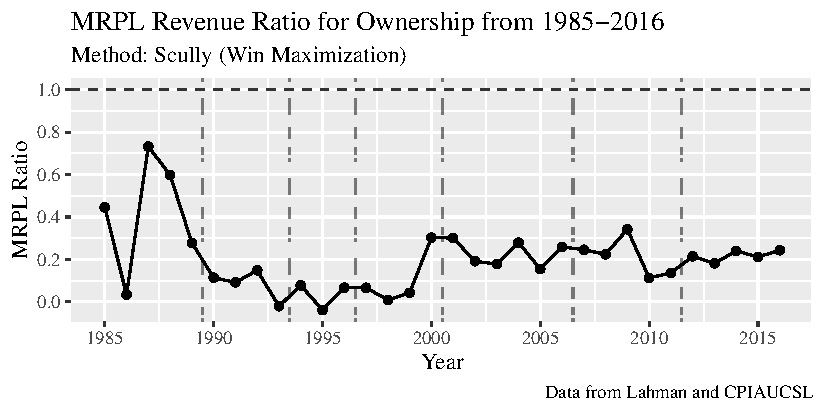
\includegraphics{FullDraft3_files/figure-pdf/fig-LeagueWPCT-1.pdf}

}

\caption{\label{fig-LeagueWPCT}MRPL Profit Ratio for Ownership from
1985-2016}

\end{figure}

\begin{figure}

{\centering 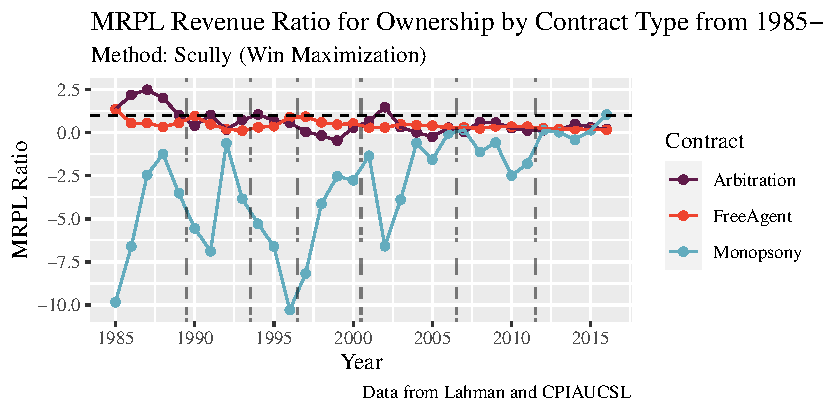
\includegraphics{FullDraft3_files/figure-pdf/fig-ContractWPCT-1.pdf}

}

\caption{\label{fig-ContractWPCT}MRPL Profit Ratio for Ownership by
Contract Type from 1985-2016}

\end{figure}

\begin{figure}

{\centering 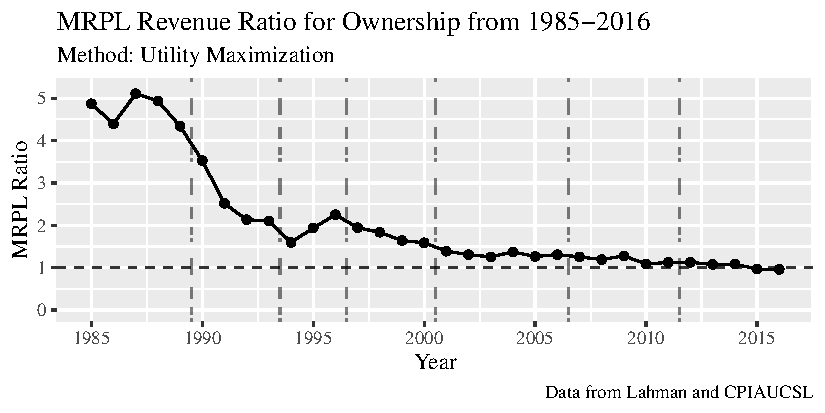
\includegraphics{FullDraft3_files/figure-pdf/fig-LeagueRSRC-1.pdf}

}

\caption{\label{fig-LeagueRSRC}MRPL Profit Ratio for Ownership from
1985-2016}

\end{figure}

\begin{figure}

{\centering 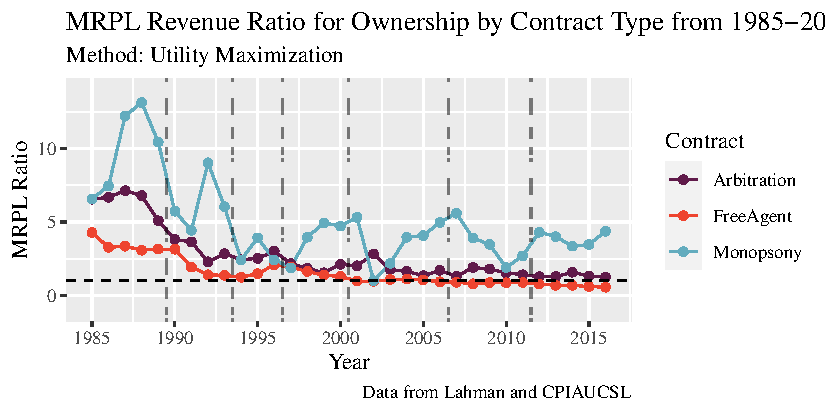
\includegraphics{FullDraft3_files/figure-pdf/fig-ContractRSRC-1.pdf}

}

\caption{\label{fig-ContractRSRC}MRPL Profit Ratio for Ownership by
Contract Type from 1985-2016}

\end{figure}



\end{document}
